date : 12 december 2023

Waar zit de start van een low power ontwerp?
\begin{itemize}
    \item In kaart brengen van de duur en piek van het vermogens verbruik
    \item fysieke grootte
    \item I/O vraag
    \item Aan/uit tijd
    \item opladen?
\end{itemize}

\vspace{0.5cm}
Wat te doen om batterij te sparen?
\begin{itemize}
    \item Geen optische interfaces.
    \item gebruik geen relais. Alleen solid state relais als het echt nodig is.
    \item geen backlight als het geen eis is.
    \item zo min mogelijk leds
    \item zo min mogelijk IO.
    \item Snelheid is een killer. Dubbele Snelheid is dubbel vermogen.
\end{itemize}

\vspace{0.5cm}
Wat kan uit\dots
\begin{itemize}
    \item Denk na over duty cycle of use.
    \item stablisatie na inschakelen?
    \item meer vermogen voor beheersing van power.
    \item zijn pull-up weerstanden altijd nodig? mag het ook met pull down?
    \item power buffers - line buffers.
    \item let op diode kruip-paadjes
    \item kunnen de
    \begin{itemize}
        \item opamps
        \item DA converters
        \item Stroombronnen
        \item Processoren
    \end{itemize}
    uit en hoe gaan ze weer aan?
\end{itemize}

\vspace{0.5cm}
Selectie vragen voeding.
\begin{itemize}
    \item Wat voor spanning is nodig?
    \item Moet de batterij oplaadbaar zijn?
    \item Hoe ziet de gebruiks/laad cycle eruit voor dit roduct?
    \item Wat is het piekverbruik van het system?
    \item Moet de batterij eenvoudig vervangbaar zijn?
    \item laden en simultaan gebruiken van de accu?
\end{itemize}

\begin{figure}[H]
    \centering
    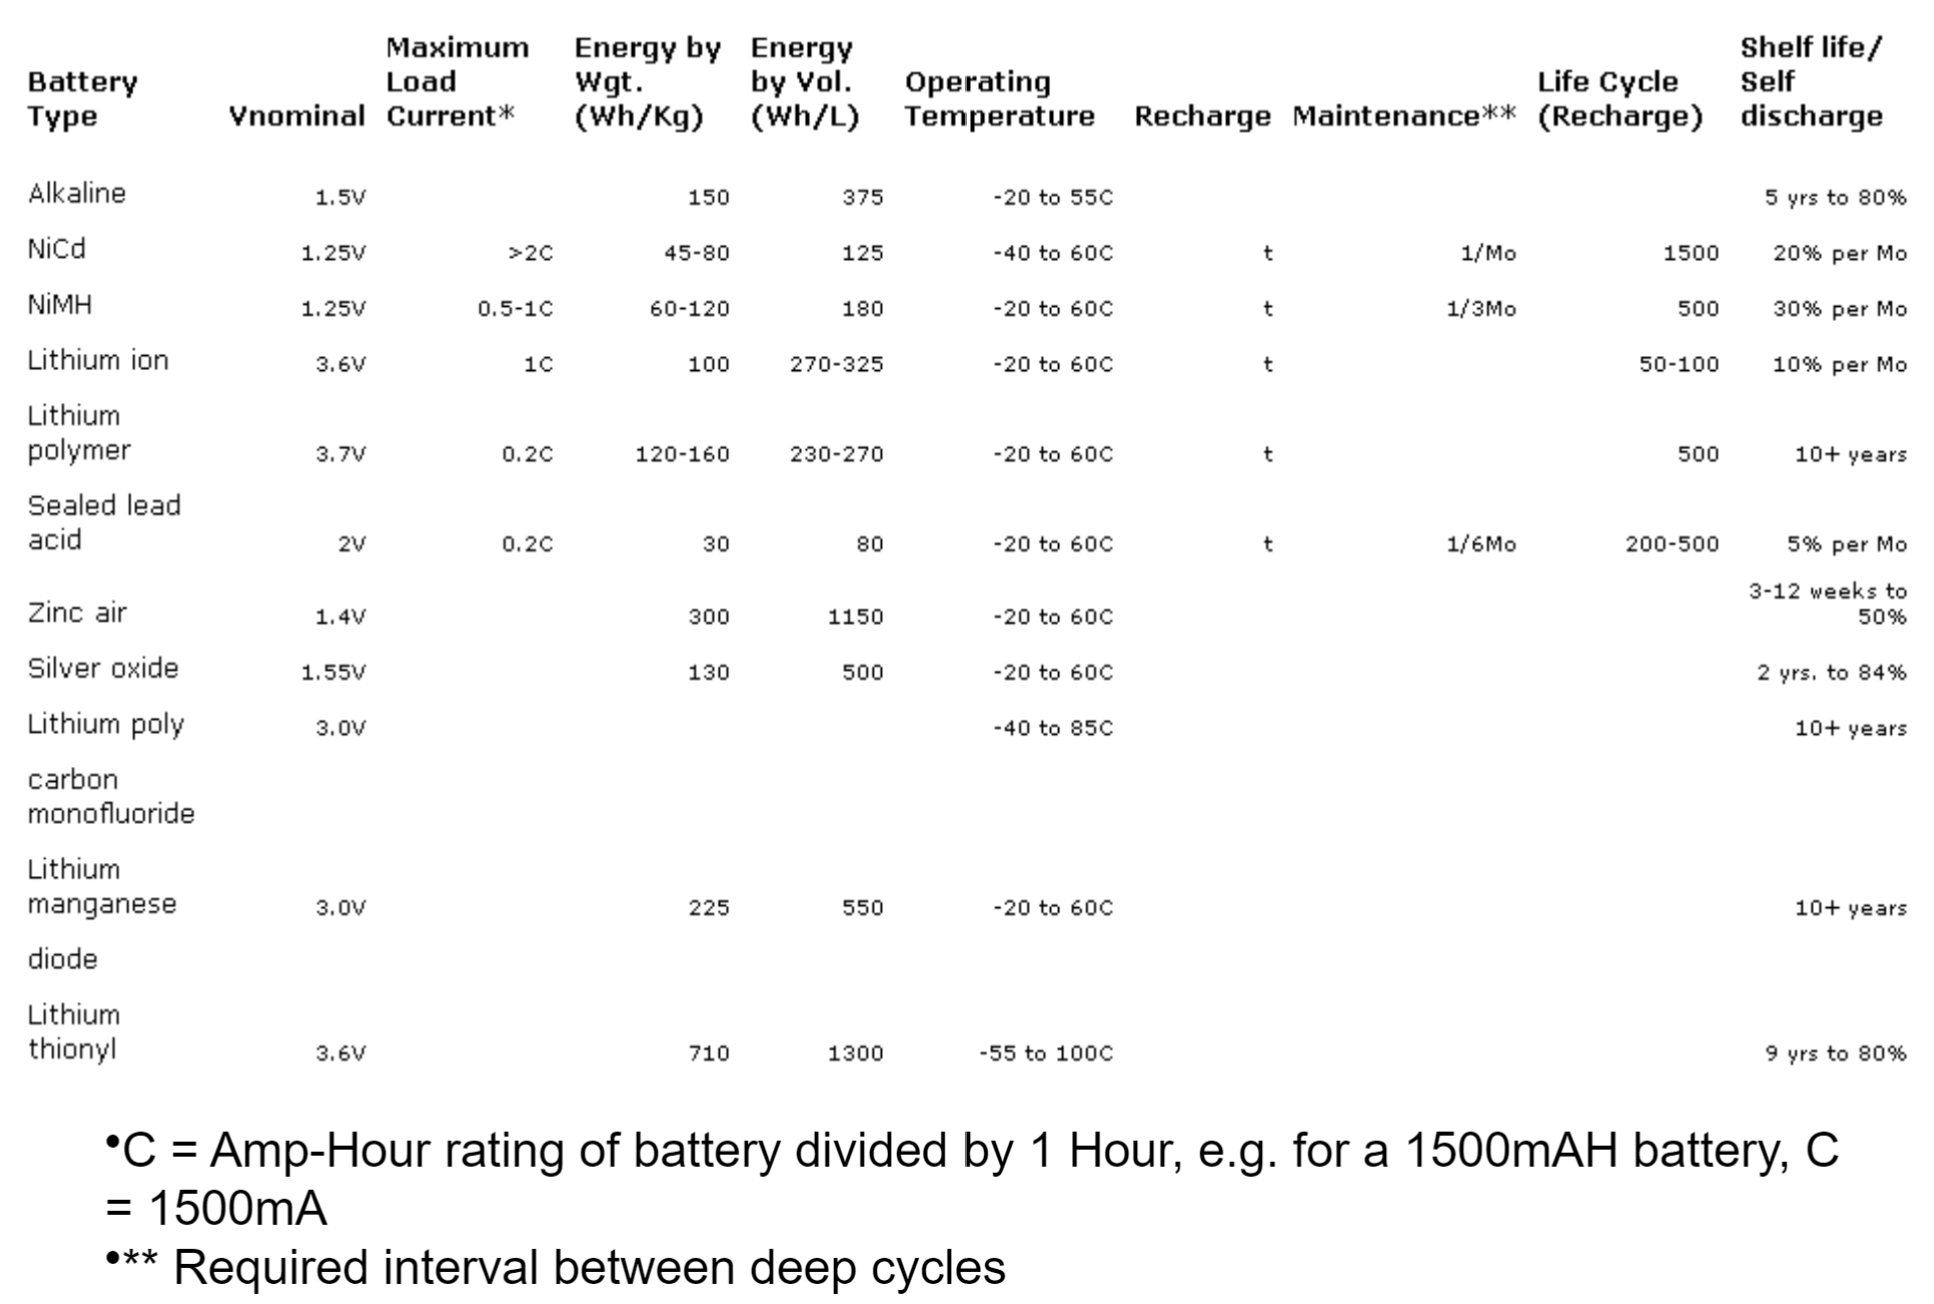
\includegraphics[scale=0.5]{batterijen.png}
    \caption*{ soorten batterijen}
    \end{figure}
